%!TEX root = ../../template.tex
%%%%%%%%%%%%%%%%%%%%%%%%%%%%%%%%%%%%%%%%%%%%%%%%%%%%%%%%%%%%%%%%%%%%
%% use_cases.tex
%% Use Cases section for Architecture and Design
%%%%%%%%%%%%%%%%%%%%%%%%%%%%%%%%%%%%%%%%%%%%%%%%%%%%%%%%%%%%%%%%%%%%

\section{Use Cases}
\label{sec:UseCases}

This section describes the use cases that define its expected behavior, and presents a use case diagram that illustrates the relationships between them. These use cases feed into the requirements specification in Section~\ref{sec:RequirementsSpecification} and, consequently, for the architectural decisions presented in the remaining sections of this chapter.

\subsection{Actors}

The platform identifies four actors, each representing a distinct role in the system:

\begin{description}
    \item[End User] Human user who interacts with the platform through the web application to manage devices, configure monitoring, and respond to alerts.
    \item[\gls{IoT} Device] Hardware device that connects to the platform and sends telemetry data.
    \item[Edge Node] Intermediate node deployed near devices that provides local monitoring capabilities and operates independently of cloud connectivity.
    \item[System] Automated platform processes that react to events without direct user interaction.
\end{description}

\subsection{Use Case Diagram}

Figure~\ref{fig:use-case-diagram} presents the use case diagram for the platform, showing the interactions between the four actors and the thirteen use cases identified.

\begin{figure}[H]
    \centering
    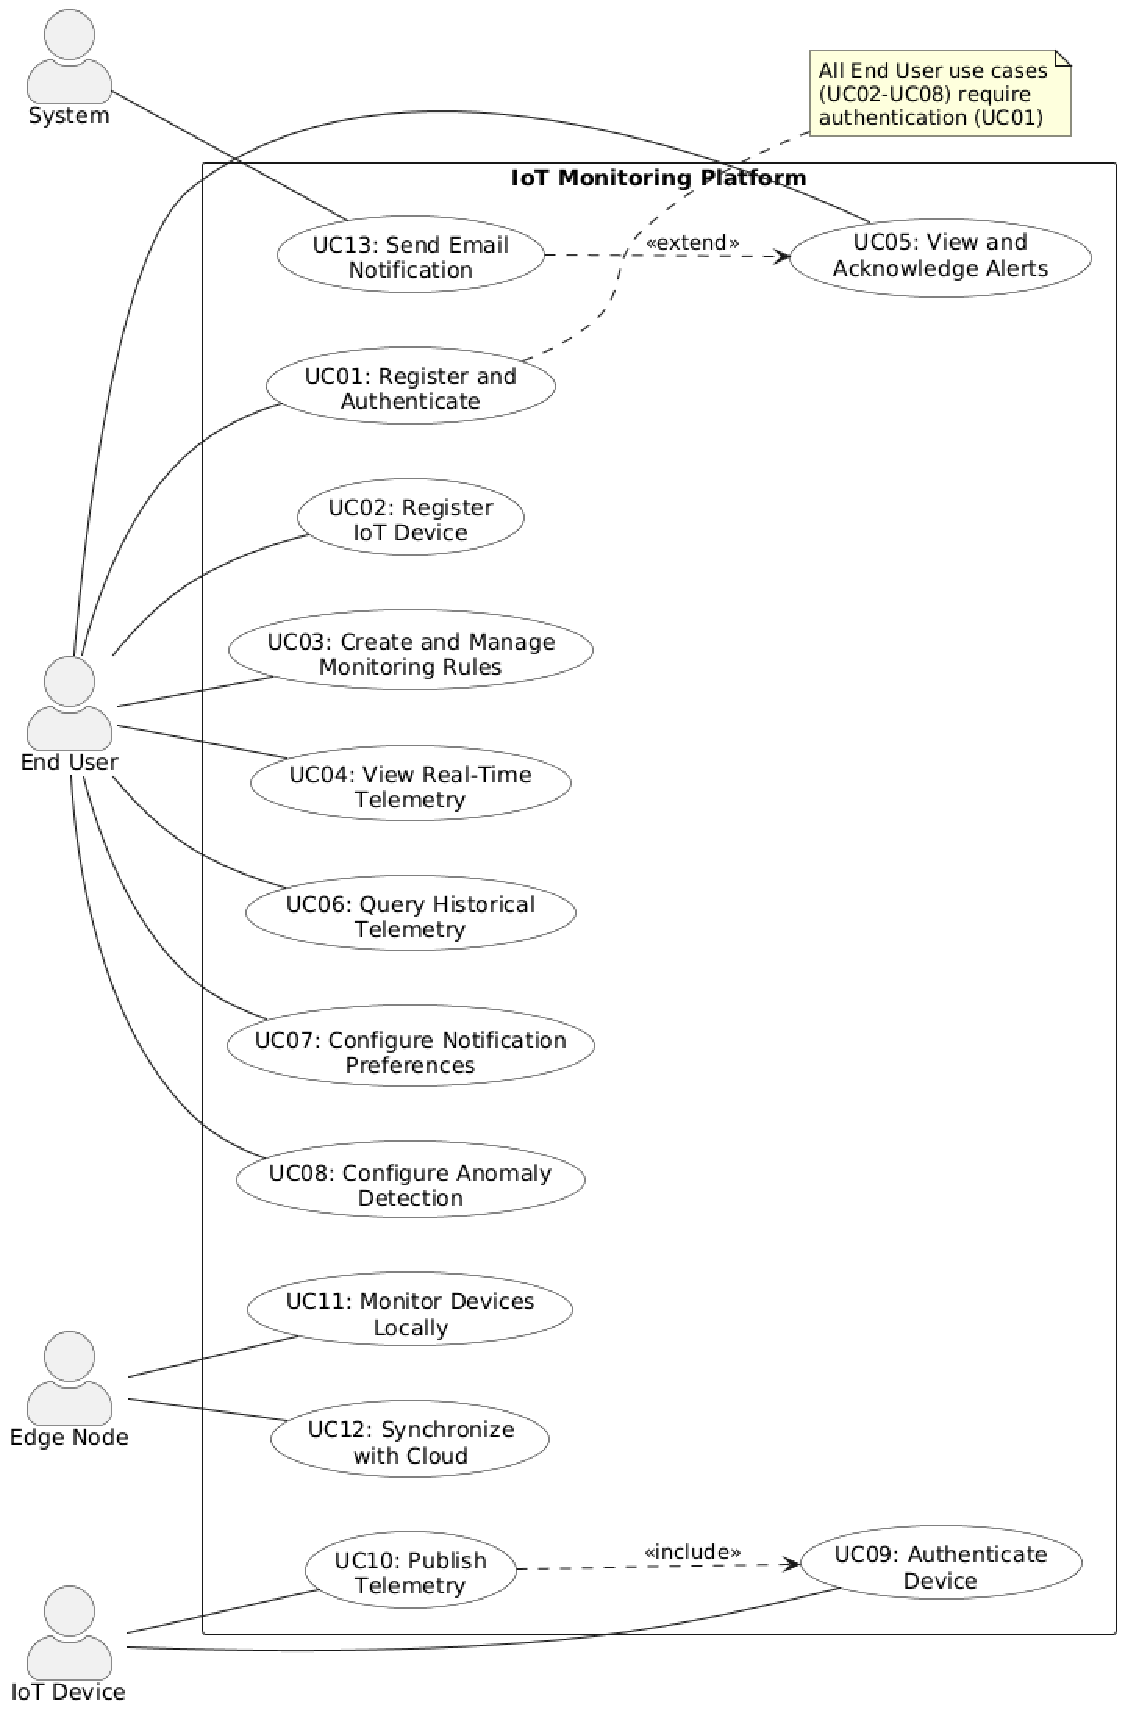
\includegraphics[width=0.8\textwidth, keepaspectratio]{Chapters/Figures/use-cases-diagram.pdf}
    \caption{Use case diagram of the \gls{IoT} monitoring platform.}
    \label{fig:use-case-diagram}
\end{figure}

\subsection{Use Case Descriptions}

Tables~\ref{tab:uc-end-user} through~\ref{tab:uc-system} describe each use case grouped by actor.

\begin{table}[H]
    \centering
    \caption{End User use cases.}
    \label{tab:uc-end-user}
    \small
    \rowcolors{2}{gray!8}{}
    \begin{tabularx}{\textwidth}{l l X}
        \toprule
        \textbf{ID} & \textbf{Name}                      & \textbf{Description}                                                                                                \\
        \midrule
        UC01        & Register and Authenticate          & Create an account and log in to access the platform.                                                                \\
        UC02        & Register \gls{IoT} Device          & Register a new device so the platform can receive and identify its telemetry.                                       \\
        UC03        & Create and Manage Monitoring Rules & Define, edit, enable, disable, or delete rules that trigger alerts when telemetry values meet specified conditions. \\
        UC04        & View Real-Time Telemetry           & Observe live telemetry from a device as it arrives.                                                                 \\
        UC05        & View and Acknowledge Alerts        & Browse generated alerts, filter them by device, severity, or status.                 \\
        UC06        & Query Historical Telemetry         & Get past telemetry for a device within a specified time range.                                                 \\
        UC07        & Configure Notification Preferences & Choose which alert severity levels trigger email notifications.                                                     \\
        UC08        & Configure Anomaly Detection        & Adjust anomaly detection sensitivity for specific devices or telemetry fields.                                      \\
        \bottomrule
    \end{tabularx}
\end{table}

\begin{table}[H]
    \centering
    \caption{\gls{IoT} Device use cases.}
    \label{tab:uc-iot-device}
    \small
    \rowcolors{2}{gray!8}{}
    \begin{tabularx}{\textwidth}{l l X}
        \toprule
        \textbf{ID} & \textbf{Name}       & \textbf{Description}                                                               \\
        \midrule
        UC09        & Authenticate Device & Identify and authenticate with the platform to establish an authorized connection. \\
        UC10        & Publish Device Data  & Send telemetry data or upload files to the platform. Includes UC09.                \\
        \bottomrule
    \end{tabularx}
\end{table}

\begin{table}[H]
    \centering
    \caption{Edge Node use cases.}
    \label{tab:uc-edge-node}
    \small
    \rowcolors{2}{gray!8}{}
    \begin{tabularx}{\textwidth}{l l X}
        \toprule
        \textbf{ID} & \textbf{Name}           & \textbf{Description}                                                                                                                   \\
        \midrule
        UC11        & Monitor Devices Locally & Receive and process telemetry from devices, evaluate rules, and generate alerts independently of cloud connectivity. \\
        UC12        & Synchronize with Cloud  & Send locally collected telemetry and alerts to the cloud platform when connectivity is available.                                   \\
        \bottomrule
    \end{tabularx}
\end{table}

\begin{table}[H]
    \centering
    \caption{System use cases.}
    \label{tab:uc-system}
    \small
    \rowcolors{2}{gray!8}{}
    \begin{tabularx}{\textwidth}{l l X}
        \toprule
        \textbf{ID} & \textbf{Name}           & \textbf{Description}                                                        \\
        \midrule
        UC13        & Send Email Notification & Notify users by email when an alert matches their notification preferences. \\
        \bottomrule
    \end{tabularx}
\end{table}

UC10 (Publish Device Data) includes UC09 (Authenticate Device), as device authentication is a prerequisite for publishing data. UC10 covers both structured \gls{JSON} telemetry and binary file uploads, since both are forms of authenticated device data ingestion. All End User use cases (UC02 through UC08) require prior authentication (UC01). UC13 (Send Email Notification) extends the alert generation triggered by rule evaluation (UC03) and anomaly detection (UC08).
